\section{Konzeptentwurf der Anwendungsarchitektur}
\label{sec:konzeptentwurf}
Bevor die Anwendung in die Cloud migriert werden kann, muss konzeptioniert werden, wie die Anwendungsarchitektur aussehen soll und wie diese funktionieren wird. Dazu wurde vorangehend in der Anforderungsanalyse herausgearbeitet, welche Merkmale eine Cloud-native Anwendung erfüllen sollte, welche Migrationsstrategie verfolgt werden kann und welche Voraussetzungen dafür geschaffen werden müssen.

\subsection{Existierender Code}
Ziel der Anwendung ist das Einsammeln der \textit{\glspl{Timesheet}}, in dem Projekt aktiver Mitarbeiter, aus einem \gls{Box}-Verzeichnis, das Überprüfen dieser und die anschließende Rechnungs- und Reporterstellung. Die Prozesse werden jeweils manuell über eine Konsoleneingabe gestartet. Im \gls{Box}-Verzeichnis liegt ein Projektmanagement-File, welcher alle Mitarbeiter enthält, die jemals in dem Projekt gearbeitet haben und markiert, welche auch aktuell aktiv sind und dem Kunden in Rechnung gestellt werden können. Außerdem sind in dem Verzeichnis auch die Reports aus einem Zeiterfassungstool abgelegt. In Abbildung \ref{fig:pmo_python} wird der Aufbau der ursprünglichen Anwendung dargestellt.

\begin{figure}[H]
    \centering
    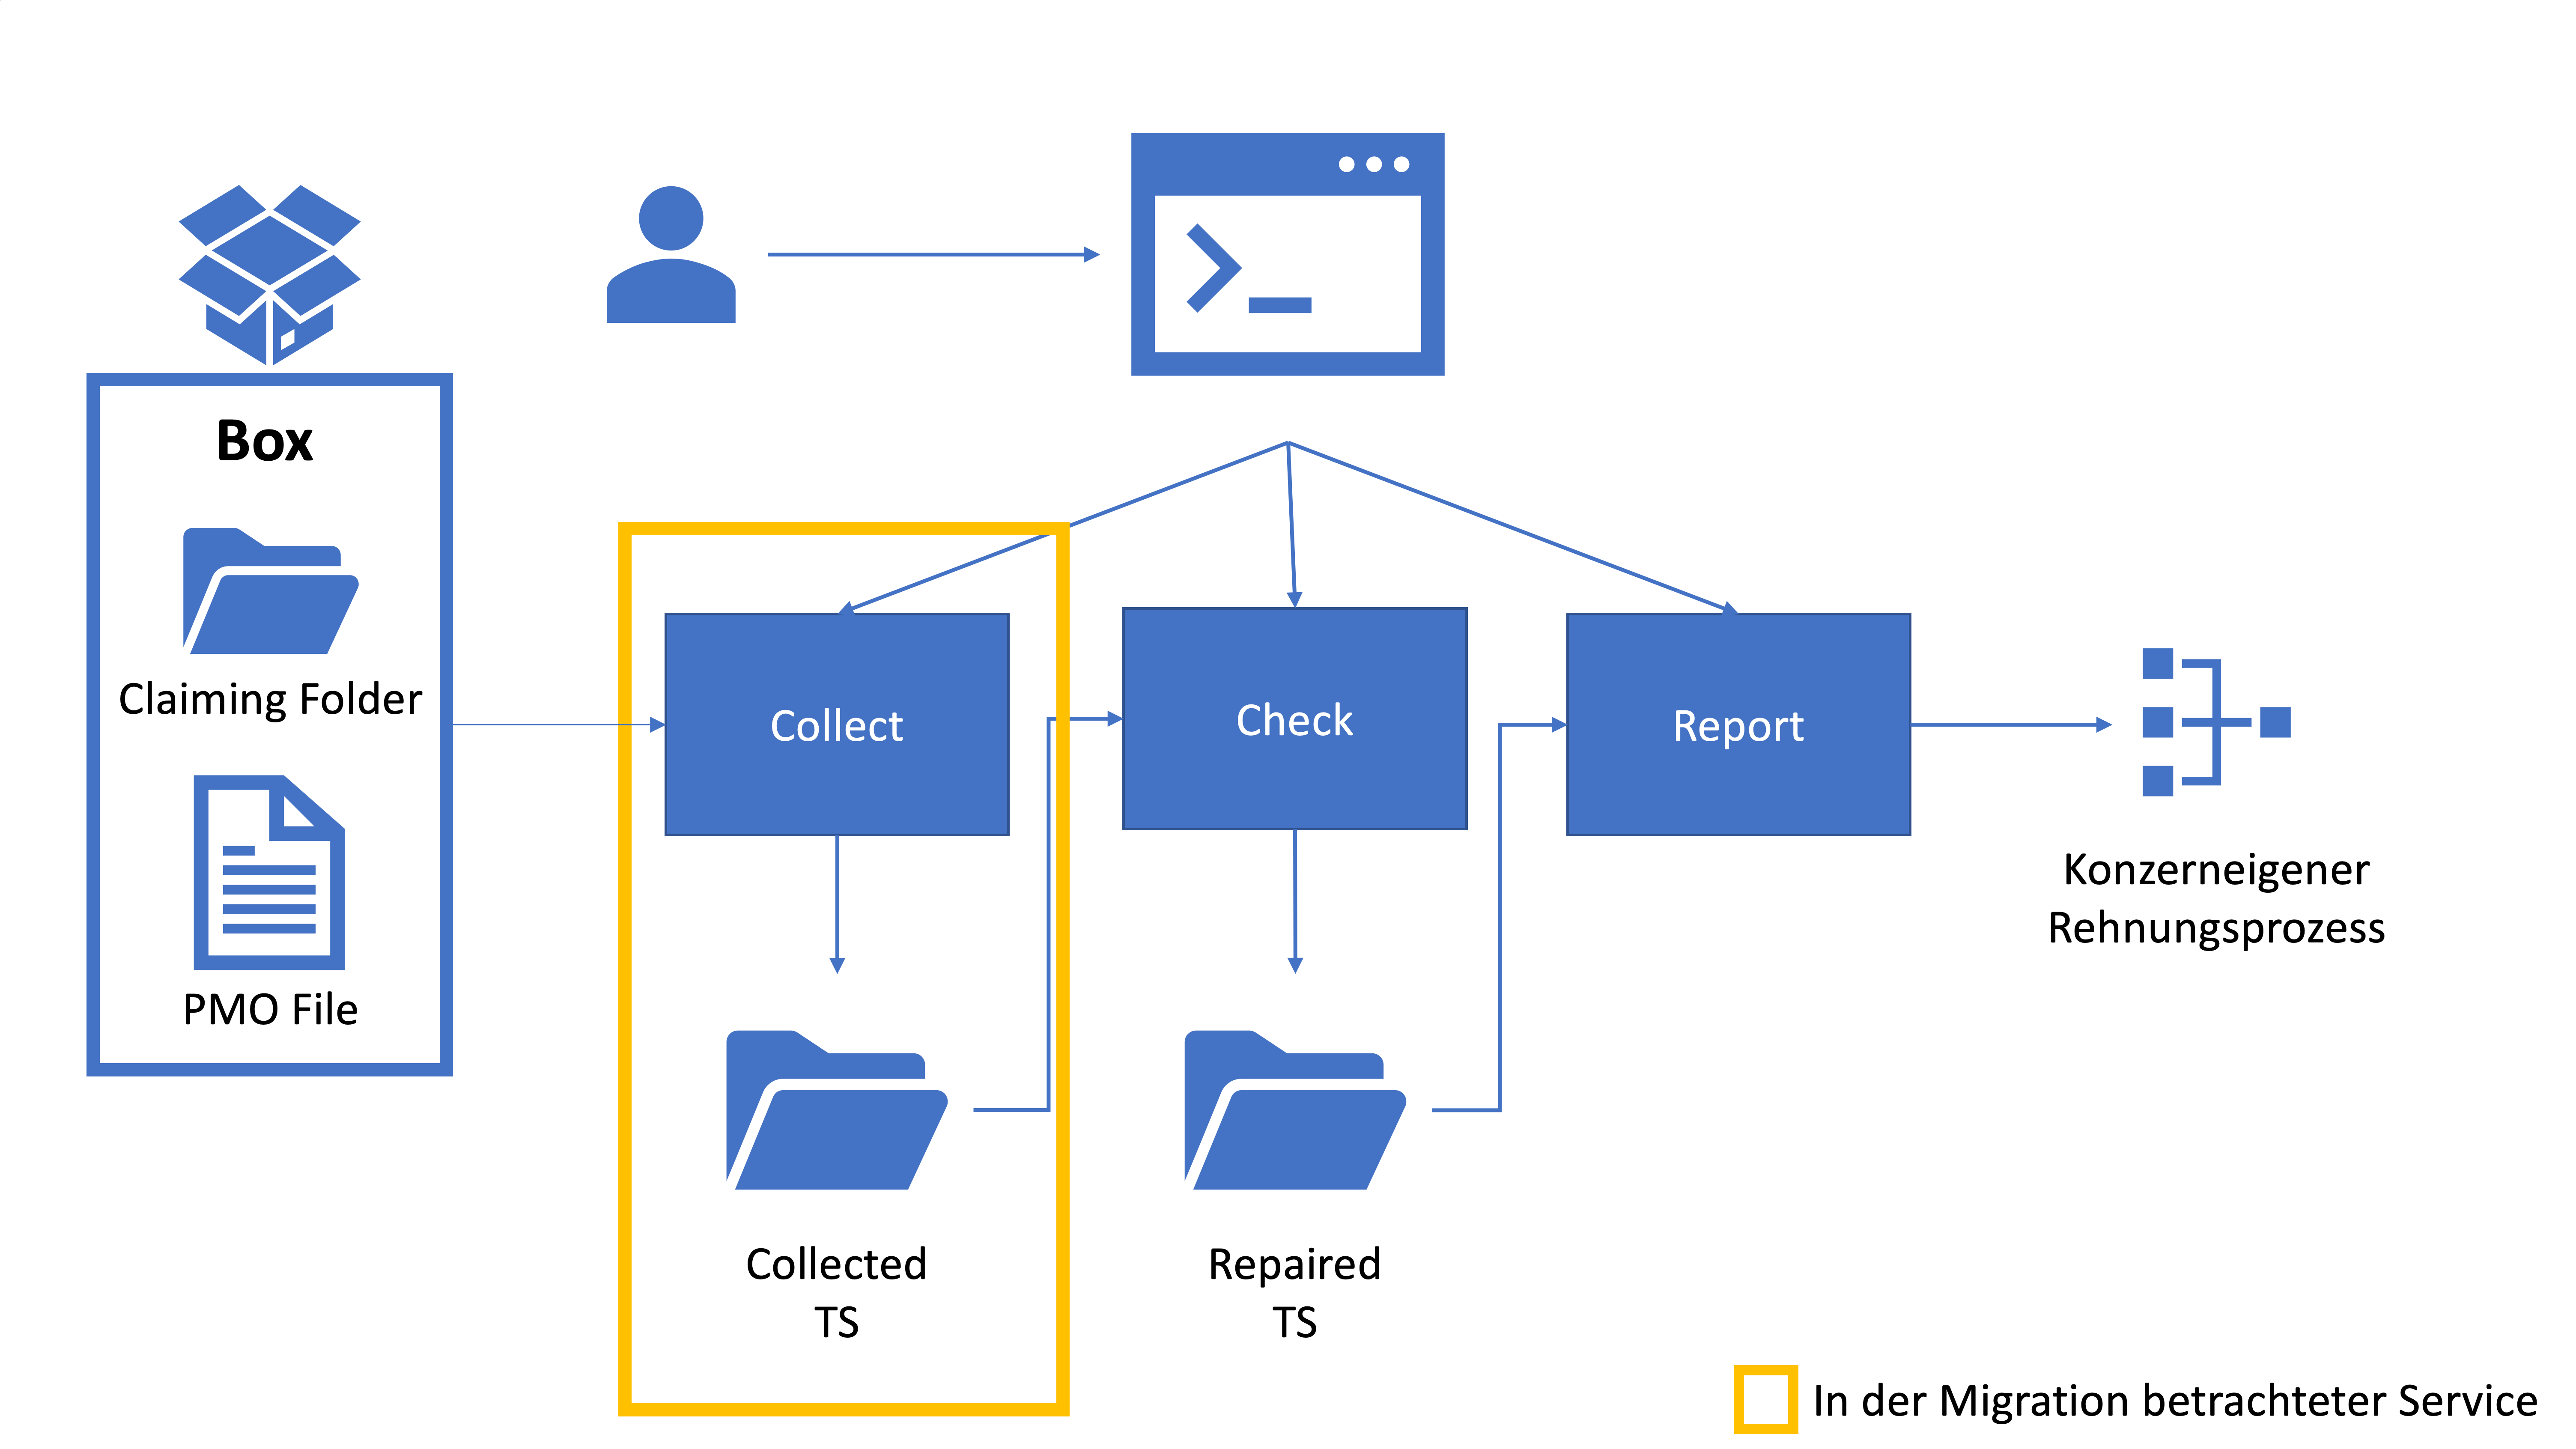
\includegraphics[width=0.65\textwidth]{pmo_python.png}
    \caption{Aufbau der ursprünglichen Anwendung (gelb umrandet der Teil, der prototypisch migriert wird)}
    \label{fig:pmo_python}
\end{figure}

Die bisher existierende Anwendung ist eine Python Anwendung, die grundsätzlich in drei Module aufgeteilt ist:
\begin{itemize}
\item \textbf{Timesheet Collector: }Einsammeln der \textit{\glspl{Timesheet}}, der in dem Projekt aktiven Mitarbeiter und Ablegen dieser in einem neuen Verzeichnis
\item \textbf{Timesheet Checker: }Überprüfen der \textit{\glspl{Timesheet}} auf Korrektheit und Vollständigkeit und gegebenenfalls Reparatur dieser (Fehlerkorrektur und Abgleich mit Daten aus Zeiterfassungstool zur Vermeidung von Unstimmigkeiten)
\item \textbf{Timesheet Report: }Erzeugung eines Berichts, Zusammenfassung der dokumentierten Stunden und Verteilung dieser auf die unterschiedlichen Beauftragungen, Erstellung von Nachweisdokumenten für die konzerneigene Rechnungsstellung
\end{itemize}

Jeder dieser drei Services ist ein eigenes Python Modul. Diese greifen jeweils auf weitere gemeinsame Services wie einen Excel-Helper und Checking-Tools zurück.

Da es sich bei dieser Arbeit um eine Machbarkeitsstudie mit Erstellung eines Prototypen handelt, wird im ersten Schritt nur die Migration des \textit{Collect Service} untersucht, bevor die anderen, komplexeren Services migriert werden. Dies ist in Abbildung \ref{fig:pmo_python} entsprechend durch den gelben Rahmen gekennzeichnet. Der \textit{Collect Service} benötigt eine Verbindung zu dem \gls{Box}-Verzeichnis und einen Ablageort für die ''eingesammelten'' \textit{\glspl{Timesheet}}.
\pagebreak

\subsection{Entwurf der neuen Architektur}
Kern der Anwendung soll trotz der Weiterentwicklung und anstehenden Änderungen die in Kapitel \ref{sec:use-case-modellierung} beschriebene Business-Logik bilden.

In der ursprünglichen Anwendung ist der Zugriff auf die \gls{Box} mithilfe eines zusätzlichen Desktop-Clients umgesetzt worden, der es ermöglicht, Verzeichnisse in \gls{Box} wie einen lokalen Dateipfad ansprechen zu können. Somit konnte der Box-Pfad in eine Konfigurationsdatei geschrieben und als Parameter an die Anwendung übergeben werden. Da in einem Container in der Cloud Umgebung kein Zugriff auf ein lokales Verzeichnis mit entsprechender \gls{Box}-Erweiterung in der selben Art und Weise hergestellt werden kann, muss hier in der neuen Anwendung entsprechend die \gls{Box}-\ac{API} eingebunden werden um den Zugriff auf die Verzeichnisse weiterhin zu ermöglichen. Insbesondere auch deshalb, weil die Mehrbenutzerfähigkeit gewährleistet werden soll, welche über ein lokales Verzeichnis nicht umsetzbar wäre. Hierfür stellt \gls{Box} selbst ein entsprechendes \ac{SDK} für diverse Sprachen bereit.

Außerdem enthalten die PMO-Tools ein Skript, welches den Umgang mit Excel Spreadsheets ermöglicht. Dazu gehört zum einen das Ermitteln aktiver Mitarbeiter und zum anderen das Auslesen der \textit{\glspl{Timesheet}}, was jedoch für den untersuchten Service vorerst keine Verwendung findet. Einen vergleichbaren Service muss auch die neue Anwendung zum Lesen des PMO-Files enthalten. Für andere Programmiersprachen, wie zum Beispiel Java kann man in diesem Fall auf \textit{Libraries} wie die \gls{Apache POI} Programmbibliothek zurückgreifen, welche das Lesen und Schreiben von Microsoft Office Dateien ermöglicht.

Den ''Hauptservice'' der Anwendung soll der \textit{\gls{Timesheet}}-Service bilden. Dieser soll alle Funktionen bereitstellen, die unter Verwendung der anderen Services die letztendlich gewünschte Funktionalität - das Einsammeln der \textit{\glspl{Timesheet}} - bieten. Darüber hinaus soll dieser für eine spätere Anwendungsversion auch die anderen Funktionalitäten aus der ursprünglichen Anwendung bereitstellen. In der ursprünglichen Anwendung wurden die Services durch eine Konsoleneingabe im Terminal gestartet. Dies ist so bei der Cloud Anwendung nicht mehr ohne weiteres möglich, weshalb die Anwendung zukünftig über einen \ac{API}-Endpunkt bereitgestellt wird. \pagebreak

Abbildung \ref{fig:Architektur} zeigt einen groben  Entwurf der Anwendung und wie die Services miteinander kommunizieren sollen. Der \textit{\gls{Timesheet}} Service soll zu einem späteren Zeitpunkt alle Funktionen aus der Ursprünglichen Anwendung bündeln, für den Prototypen wird sich jedoch, wie bereits in der Anforderungsanalyse erwähnt, auf den \textit{Collect Service} beschränkt.

\begin{figure}[H]
    \centering
    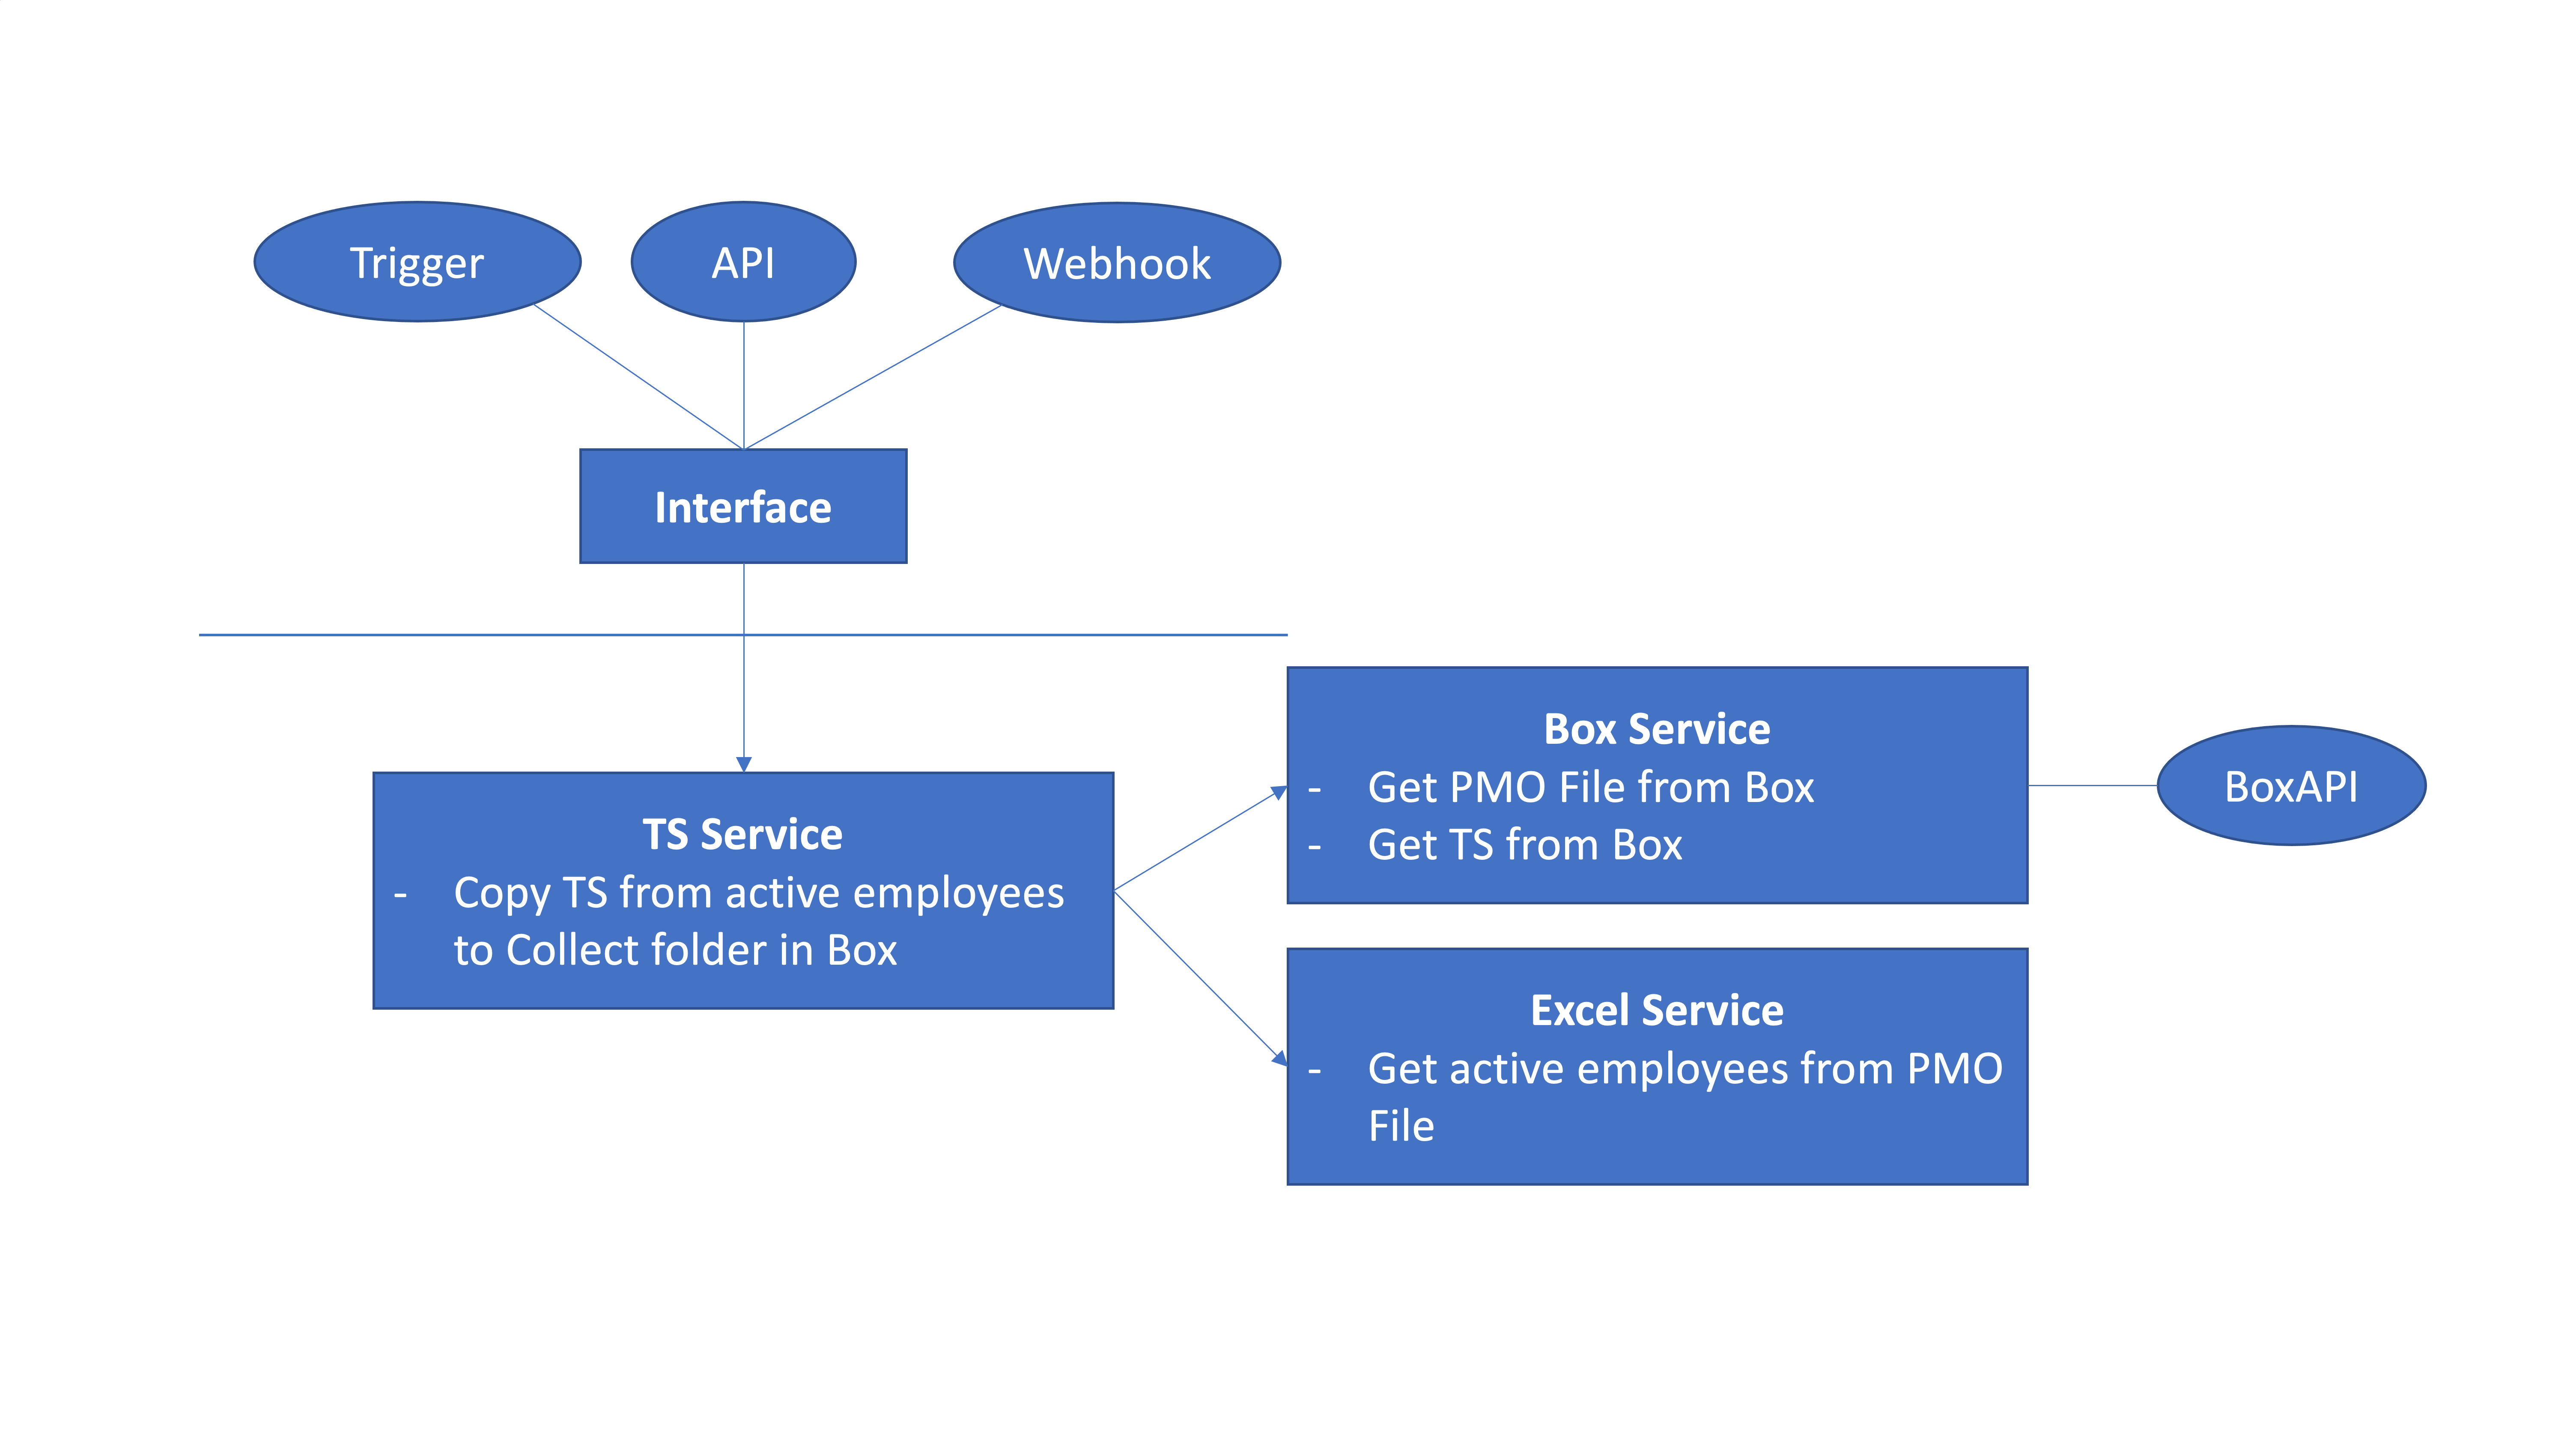
\includegraphics[width=\textwidth]{architektur.png}
    \caption{Architekturentwurf der neuen Anwendung}
    \label{fig:Architektur}
\end{figure}

In dem Prototypen wird die Anwendung über eine \ac{API} bereitgestellt werden. \textit{Trigger}\footnote{dt. Auslöser, z. B. durch Hochladen einer neuen Konfigurationsdatei} und \textit{Webhook}\footnote{Eigenwort, z. B. durch \gls{Box}-API bereitgestellte Verknüpfung zur Überwachung eines Ordners, Funktion ähnlich zu Trigger}, wie in der Abbildung dargestellt, sollen visualisieren, dass auch alternative Interfaces eingesetzt werden können, ohne die Funktionalität der Anwendung zu beeinflussen. Neben der Erfüllung dieser funktionalen Anforderungen sollen auch die nicht-funktionalen Aspekte betrachtet werden. Dazu gehören die in Kapitel \ref{sec:anforderungsanalyse} erarbeiteten Anforderungen an eine Cloud-native Anwendung, unter anderem die Skalierbarkeit und Fehlertoleranz. Diese sollen über die in Kapitel \ref{sec:cloud-infra} konzipierte Cloud Infrastruktur in \ac{AWS} ermöglicht werden. \pagebreak

\subsection{Programmiersprache und Framework}
% Dependecy Injektion sehr gut (Austauschbarkeit der Implementierung)
% Spring MVC für REST-Anwendung in Springboot enthalten (Teil des Spring-Frameworks)
Neben der Konzeptionierung einer Anwendungsarchitektur braucht es zur Entwicklung auch eine Programmiersprache und gegebenenfalls ein Framework, um die Anwendung optimal in der Cloud beziehungsweise als Web-Anwendung nutzen zu können. 

Im Falle der PMO-Tools wurde ursprünglich Python verwendet, jedoch erschien im Zuge des Refactoring ein Wechsel zu Java und dem \gls{Spring} Framework sinnvoll, da hier mit \gls{Spring Boot} die Cloud-native Entwicklung erleichtert wird. Darüber hinaus gilt \gls{Spring Boot} als populärer Standard für den Einsatz von Microservices und die Bereitstellung einer \ac{REST}-\ac{API} ist mit \gls{Spring Boot} einfacher umzusetzen, da mit \textit{Spring MVC} bereits ein Web-Framework in \gls{Spring} enthalten ist, zur Bereitstellung von \ac{REST}-Endpunkten.

\subsection{Auswahl eines Cloud Providers}
Ein für die Cloud Migration unerlässlicher Schritt ist die Auswahl eines zu den Anforderungen passenden Cloud Providers. In diesem Fall wurde \ac{AWS} als einer der größten Provider \cite[Vgl.][S. 6]{Sustar2022} gewählt, da hier mit \ac{ECS} und \gls{Fargate} gute Möglichkeiten zur \textit{serverless} Bereitstellung von Containern zur Verfügung stehen um somit die Vorteile der Cloud optimal nutzen zu können. Darüber hinaus unterstützt \ac{AWS} viele offene Standards und Open-Source Tools, wie zum Beispiel \ac{IaC} mit Terraform.

Alternativ wurden auch die Services der IBM-Cloud in Betracht gezogen, da hier mit \textit{Cloud Functions} oder \textit{CodeEngine} ebenfalls Plattformen zur Bereitstellung von Containern existieren, die jedoch zum einen schwieriger aufzusetzen schienen und zum anderen bezüglich der Möglichkeiten nicht mit \ac{ECS} vergleichbar sind. Ebenfalls hätte Azure, die Cloud Plattform von Microsoft, infrage kommen können, da jedoch \ac{AWS} auch im Projektumfeld eingesetzt wird, wurde diese Alternative bevorzugt. \pagebreak